Der Schertest ist ein Verfahren zur Untersuchung der mechanischen Festigkeit von Verbindungen zwischen unterschiedlichen Materialien.  Er kommt besonders dann zum Einsatz, wenn die Belastbarkeit von Bindemitteln bewertet werden soll, die beispielsweise Metall- oder Kunststoffkomponenten miteinander verbinden.\\

Bei der Durchführung eines Schertests werden Prüfkörper, bestehend aus mehreren Scherkörpern, auf einer Bodenplatte befestigt. Mithilfe eines Schermeißels wird eine seitlich wirkende Kraft aufgebracht, die die Scherkörper kontrolliert abschert. Dabei wird sowohl die aufgewendete Kraft als auch der Weg des Meißels aufgezeichnet, um daraus ein Kraft-Weg-Diagramm zu erstellen.\\

Die zentrale Messgröße ist die mittlere Haftfestigkeit, die durch Umrechnung der gemessenen Kraft auf die Querschnittsfläche der Scherkörper N/mm² bestimmt wird.  \\

Zur statistischen Auswertung der Ergebnisse wird ein Boxplot-Diagramm erstellt. Dieses zeigt nicht nur die Verteilung der ermittelten Haftfestigkeiten, sondern erlaubt auch den direkten Vergleich verschiedener Prüfkörper. Daraus können im Endeffekt Brucharten verglichen werden, um die Art des Versagens genauer zu klassifizieren etwa als adhäsiv, kohäsiv oder gemischt.\\
Die Prüfkörper werden auf Widerstand untersucht, dieser Widerstand sagt uns wie viel Schubspannung ein Scherkörper aufnehmen kann bis Scherabriss sich bildet.\\
Es gilt folgende Formel zur Berechnung der Schubspannung:\\
\begin{equation}
    \tau = \frac{F}{A}
\end{equation}   
\vspace{0.2cm}
\begin{figure}
    \centering
    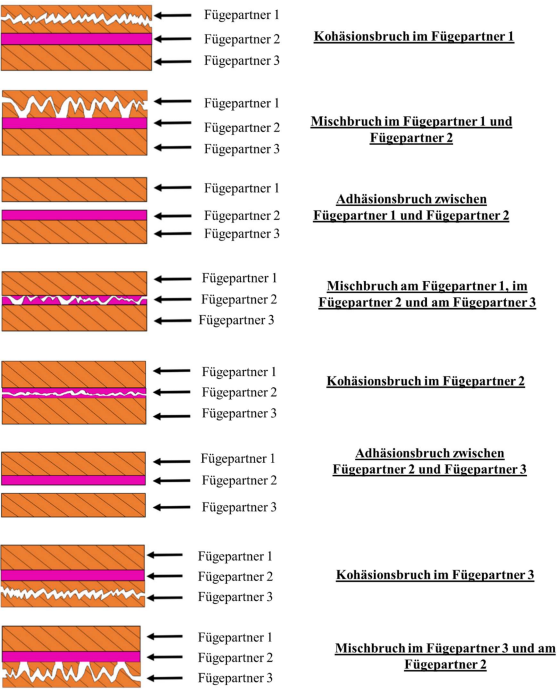
\includegraphics{Bilder/Brucharten.png}
    \caption{Mögliche Bruchbilder eines Schertests}
    \caption*{\textit{Quelle: https://tinyurl.com/2p8ejcnv }}
    \vspace{0.2cm}
    \label{Abb.3: Mögliche Bruchbilder eines Schertests}
\end{figure}
\\
